\section{Date: 2026-11-12}
\noindent \textbf{Series ID: EEMXSLNQ} 

\noindent This series is titled Weighted-Average Effective Loan Rate for 31 to 365 Days, Large Domestic Banks (DISCONTINUED) and has a frequency of Quarterly, 2nd Month's 1st Full Week. The units are Percent and the seasonal adjustment is Not Seasonally Adjusted.The observation start date is 1997-04-01 and the observation end date is 2017-04-01.The popularity of this series is 1. \\ 

\noindent \textbf{Series ID: CXU190904LB0902M} 

\noindent This series is titled Expenditures: Food Prepared on Out-of-Town Trips by Race: White, Asian, and All Other Races, Not Including Black or African American and has a frequency of Annual. The units are U.S. Dollars and the seasonal adjustment is Not Seasonally Adjusted.The observation start date is 1984-01-01 and the observation end date is 2024-01-01.The popularity of this series is 1. \\ 

\subsection{Raw Regression}
\noindent Regresses the two series against each other directly. A significant result here can come just as easily from both series sharing a long-run trend as from any real relationship.

\begin{center}
\begin{tabular}{lclc}
\toprule
\textbf{Dep. Variable:}        & value\_fred\_CXU190904LB0902M & \textbf{  R-squared:         } &     0.146   \\
\textbf{Model:}                &              OLS              & \textbf{  Adj. R-squared:    } &     0.098   \\
\textbf{Method:}               &         Least Squares         & \textbf{  F-statistic:       } &     3.067   \\
\textbf{Date:}                 &        Thu, 12 Nov 2026       & \textbf{  Prob (F-statistic):} &   0.0969    \\
\textbf{Time:}                 &            19:16:13           & \textbf{  Log-Likelihood:    } &   -63.734   \\
\textbf{No. Observations:}     &                 20            & \textbf{  AIC:               } &     131.5   \\
\textbf{Df Residuals:}         &                 18            & \textbf{  BIC:               } &     133.5   \\
\textbf{Df Model:}             &                  1            & \textbf{                     } &             \\
\textbf{Covariance Type:}      &           nonrobust           & \textbf{                     } &             \\
\bottomrule
\end{tabular}
\begin{tabular}{lcccccc}
                               & \textbf{coef} & \textbf{std err} & \textbf{t} & \textbf{P$> |$t$|$} & \textbf{[0.025} & \textbf{0.975]}  \\
\midrule
\textbf{const}                 &      55.7666  &        3.676     &    15.170  &         0.000        &       48.043    &       63.490     \\
\textbf{value\_fred\_EEMXSLNQ} &      -1.3252  &        0.757     &    -1.751  &         0.097        &       -2.915    &        0.265     \\
\bottomrule
\end{tabular}
\begin{tabular}{lclc}
\textbf{Omnibus:}       &  0.657 & \textbf{  Durbin-Watson:     } &    0.875  \\
\textbf{Prob(Omnibus):} &  0.720 & \textbf{  Jarque-Bera (JB):  } &    0.646  \\
\textbf{Skew:}          &  0.105 & \textbf{  Prob(JB):          } &    0.724  \\
\textbf{Kurtosis:}      &  2.145 & \textbf{  Cond. No.          } &     13.4  \\
\bottomrule
\end{tabular}
%\caption{OLS Regression Results}
\end{center}

Notes: \newline
 [1] Standard Errors assume that the covariance matrix of the errors is correctly specified.

\begin{figure}
\centering
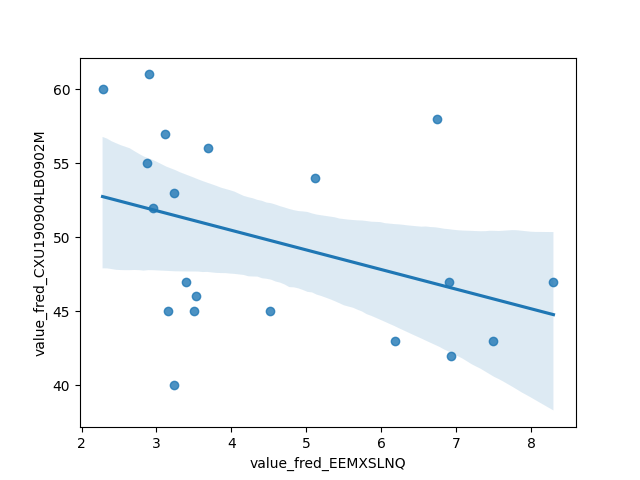
\includegraphics[scale = 0.9]{plots/plot_2026-11-12.png}
\caption{Raw Regression Plot for 2026-11-12}
\end{figure}
\newpage
\subsection{Detrended Regression}
\noindent Regresses the residuals of each series after removing its own linear time trend, so a shared trend can no longer drive the result on its own. A relationship that stays significant here is better evidence of a genuine link between the two series.

\begin{center}
\begin{tabular}{lclc}
\toprule
\textbf{Dep. Variable:}                   & value\_fred\_CXU190904LB0902M\_detrended & \textbf{  R-squared:         } &     0.006   \\
\textbf{Model:}                           &                   OLS                    & \textbf{  Adj. R-squared:    } &    -0.049   \\
\textbf{Method:}                          &              Least Squares               & \textbf{  F-statistic:       } &    0.1149   \\
\textbf{Date:}                            &             Thu, 12 Nov 2026             & \textbf{  Prob (F-statistic):} &    0.739    \\
\textbf{Time:}                            &                 19:16:13                 & \textbf{  Log-Likelihood:    } &   -59.471   \\
\textbf{No. Observations:}                &                      20                  & \textbf{  AIC:               } &     122.9   \\
\textbf{Df Residuals:}                    &                      18                  & \textbf{  BIC:               } &     124.9   \\
\textbf{Df Model:}                        &                       1                  & \textbf{                     } &             \\
\textbf{Covariance Type:}                 &                nonrobust                 & \textbf{                     } &             \\
\bottomrule
\end{tabular}
\begin{tabular}{lcccccc}
                                          & \textbf{coef} & \textbf{std err} & \textbf{t} & \textbf{P$> |$t$|$} & \textbf{[0.025} & \textbf{0.975]}  \\
\midrule
\textbf{const}                            &     8.18e-13  &        1.116     &  7.33e-13  &         1.000        &       -2.344    &        2.344     \\
\textbf{value\_fred\_EEMXSLNQ\_detrended} &       0.2713  &        0.800     &     0.339  &         0.739        &       -1.410    &        1.952     \\
\bottomrule
\end{tabular}
\begin{tabular}{lclc}
\textbf{Omnibus:}       & 12.805 & \textbf{  Durbin-Watson:     } &    1.392  \\
\textbf{Prob(Omnibus):} &  0.002 & \textbf{  Jarque-Bera (JB):  } &   11.742  \\
\textbf{Skew:}          &  1.280 & \textbf{  Prob(JB):          } &  0.00282  \\
\textbf{Kurtosis:}      &  5.745 & \textbf{  Cond. No.          } &     1.39  \\
\bottomrule
\end{tabular}
%\caption{OLS Regression Results}
\end{center}

Notes: \newline
 [1] Standard Errors assume that the covariance matrix of the errors is correctly specified.

\begin{figure}
\centering
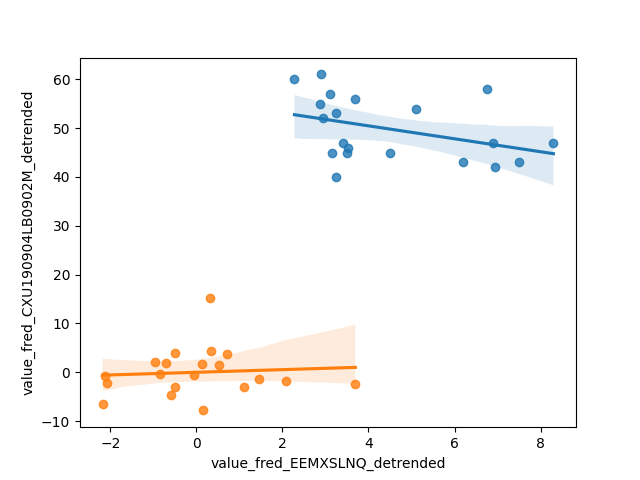
\includegraphics[scale = 0.9]{plots/plot_2026-11-12_detrended.png}
\caption{Detrended Regression Plot for 2026-11-12}
\end{figure}
\newpage
